\let\negmedspace\undefined
\let\negthickspace\undefined
\documentclass[journal,12pt,onecolumn]{IEEEtran}
\usepackage{cite}
\usepackage{amsmath,amssymb,amsfonts,amsthm}
\usepackage{algorithmic}
\usepackage{graphicx}
\graphicspath{{./figs/}}
\usepackage{textcomp}
\usepackage{xcolor}
\usepackage{txfonts}
\usepackage{listings}
\usepackage{enumitem}
\usepackage{mathtools}
\usepackage{gensymb}
\usepackage{comment}
\usepackage{mhchem}
\usepackage{caption}
\usepackage[breaklinks=true]{hyperref}
\usepackage{tkz-euclide} 
\usepackage{listings}
\usepackage{gvv}                                        
%\def\inputGnumericTable{}                                   
\usepackage[utf8]{inputenc}     
\usepackage{xparse}
\usepackage{color}                                            
\usepackage{array}                                            
\usepackage{longtable}                                       
\usepackage{calc}                                             
\usepackage{multirow}
\usepackage{multicol}
\usepackage{hhline}                                           
\usepackage{ifthen}                                           
\usepackage{lscape}
\usepackage{tabularx}
\usepackage{array}
\usepackage{float}
\newtheorem{theorem}{Theorem}[section]
\newtheorem{problem}{Problem}
\newtheorem{proposition}{Proposition}[section]
\newtheorem{lemma}{Lemma}[section]
\newtheorem{corollary}[theorem]{Corollary}
\newtheorem{example}{Example}[section]
\newtheorem{definition}[problem]{Definition}
\newcommand{\BEQA}{\begin{eqnarray}}
\newcommand{\EEQA}{\end{eqnarray}}
\newcommand{\define}{\stackrel{\triangle}{=}}
\theoremstyle{remark}
\newtheorem{rem}{Remark}

\usepackage{enumitem}
\setlist[enumerate,1]{label=\arabic*.}
\setlist[enumerate,2]{label=(\Alph*)}


\begin{document}

\title{
 GATE 2010 \\
XL: Life Sciences}
\author{EE25BTECH11049 - Sai Krishna Bakki}
\date{}
\maketitle
\begin{enumerate}

\item The question below consists of a pair of related words followed by four pairs of words. 
Select the pair that best expresses the relation in the original pair.  
\textbf{Unemployed : Worker}  

\hfill{\brak{\text{GATE XL 2010}}}

\begin{enumerate}
\begin{multicols}{2}
\item fallow : land  
\item unaware : sleeper  
\item wit : jester  
\item renovated : house  
\end{multicols}
\end{enumerate}

\item Choose the most appropriate word from the options given below to complete the following sentence:  

His rather casual remarks on politics \underline{\hspace{2cm}} his lack of seriousness about the subject.  

\hfill{\brak{\text{GATE XL 2010}}}

\begin{enumerate}
\begin{multicols}{2}
\item masked  
\item belied  
\item betrayed  
\item suppressed  
\end{multicols}
\end{enumerate}

\item Which of the following options is the closest in meaning to the word below: \\ 
\textbf{Circuitous}  

\hfill{\brak{\text{GATE XL 2010}}}

\begin{enumerate}
\begin{multicols}{2}
\item cyclic  
\item indirect  
\item confusing  
\item crooked  
\end{multicols}
\end{enumerate}

\item $25$ persons are in a room. $15$ of them play hockey, $17$ of them play football and $10$ of them play both hockey and football. 
Then the number of persons playing neither hockey nor football is  

\hfill{\brak{\text{GATE XL 2010}}}

\begin{enumerate}
\begin{multicols}{2}
\item $2$  
\item $17$  
\item $13$  
\item $3$  
\end{multicols}
\end{enumerate}

\item Choose the most appropriate word from the options given below to complete the following sentence:  

If we manage to \underline{\hspace{2cm}} our natural resources, we would leave a better planet for our children.  

\hfill{\brak{\text{GATE XL 2010}}}

\begin{enumerate}
\begin{multicols}{2}
\item rebuild  
\item restrain  
\item cherish  
\item conserve  
\end{multicols}
\end{enumerate}

\item $5$ skilled workers can build a wall in $20$ days; $8$ semi-skilled workers can build a wall in $25$ days; $10$ unskilled workers can build a wall in $30$ days. If a team has $2$ skilled, $6$ semi-skilled and $5$ unskilled workers, how long will it take to build the wall?  

\hfill{\brak{\text{GATE XL 2010}}}

\begin{enumerate}
\begin{multicols}{4}
\item $20$ days  
\item $18$ days  
\item $16$ days  
\item $15$ days  
\end{multicols}
\end{enumerate}

\item Given digits $2,2,3,3,3,4,4,4,4$, how many distinct $4$ digit numbers greater than $3000$ can be formed?  

\hfill{\brak{\text{GATE XL 2010}}}

\begin{enumerate}
\begin{multicols}{4}
\item $50$  
\item $51$  
\item $52$  
\item $54$  
\end{multicols}
\end{enumerate}

\item If $137 + 276 = 435$ how much is $731 + 672$?  

\hfill{\brak{\text{GATE XL 2010}}}

\begin{enumerate}
\begin{multicols}{4}
\item $534$  
\item $1403$  
\item $1623$  
\item $1513$  
\end{multicols}
\end{enumerate}

\item Hari \brak{H}, Gita \brak{G}, Irfan \brak{I} and Saira \brak{S} are siblings \brak{\text{i.e. brothers and sisters}}. All were born on $1^{\text{st}}$ January. The age difference between any two successive siblings \brak{\text{that is born one after another}} is less than $3$ years. Given the following facts:  

i. Hari’s age $+$ Gita’s age $>$ Irfan’s age $+$ Saira’s age.  

ii. The age difference between Gita and Saira is $1$ year. However, Gita is not the oldest and Saira is not the youngest.  

iii. There are no twins.  

In what order were they born \brak{\text{oldest first}}?  

\hfill{\brak{\text{GATE XL 2010}}}

\begin{enumerate}
\begin{multicols}{2}
\item HSGI  
\item SGHI  
\item IGSH  
\item IHSG  
\end{multicols}
\end{enumerate}

\item Modern warfare has changed from large scale clashes of armies to suppression of civilian populations. Chemical agents that do their work silently appear to be suited to such warfare; and regretfully, there exist people in military establishments who think that chemical agents are useful tools for their cause.  

Which of the following statements best sums up the meaning of the above passage:  

\hfill{\brak{\text{GATE XL 2010}}}

\begin{enumerate}
\item Modern warfare has resulted in civil strife.  
\item Chemical agents are useful in modern warfare.  
\item Use of chemical agents in warfare would be undesirable.  
\item People in military establishments like to use chemical agents in war.  
\end{enumerate}

\item For a spontaneous process, the total entropy change $\brak{\Delta S_{\text{system}} + \Delta S_{\text{surroundings}}}$ is  

\hfill{\brak{\text{GATE XL 2010}}}

\begin{enumerate}
\begin{multicols}{2}
\item equal to zero  
\item greater than zero  
\item less than zero for endothermic process  
\item less than zero for exothermic process  
\end{multicols}
\end{enumerate}

\item A battery delivers a steady current of $1.25 \, A$ for $90$ minutes. The total charge $Q$ \brak{\text{in Coulomb units}} is  

\hfill{\brak{\text{GATE XL 2010}}}

\begin{enumerate}
\begin{multicols}{4}
\item $6750$  
\item $1012.5$  
\item $112.5$  
\item $12.5$  
\end{multicols}
\end{enumerate}

\item Molecule that has no lone pair of electrons on the central atom \brak{\text{among the choices}} is  

\hfill{\brak{\text{GATE XL 2010}}}

\begin{enumerate}
\begin{multicols}{4}
\item XeF$_4$  
\item PF$_5$  
\item ClF$_3$  
\item BF$_3$  
\end{multicols}
\end{enumerate}

\item The oxidation state of nickel atom in the coordination compound $\brak{\text{Ni(NH}_3\text{)}_6\text{Cl}_2}$ is  

\hfill{\brak{\text{GATE XL 2010}}}

\begin{enumerate}
\begin{multicols}{4}
\item $-1$  
\item $0$  
\item $+1$  
\item $+2$  
\end{multicols}
\end{enumerate}

\item The compound that is aromatic, among the choices, is  

\hfill{\brak{\text{GATE XL 2010}}}
\begin{enumerate}
\item 
\begin{figure}[h!]
\centering

\includegraphics[width=0.2\columnwidth]{fig1.png}
\caption*{}
\label{fig:a5a}
\end{figure}

\item 
\begin{figure}[h!]
\centering

\includegraphics[width=0.2\columnwidth]{fig2.png}
\caption*{}
\label{fig:a5b}
\end{figure}

\item 
\begin{figure}[h!]
\centering
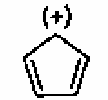
\includegraphics[width=0.2\columnwidth]{fig3.png}
\caption*{}
\label{fig:a5c}
\end{figure}

\item 
\begin{figure}[h!]
\centering
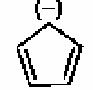
\includegraphics[width=0.2\columnwidth]{fig4.png}
\caption*{}
\label{fig:a5d}
\end{figure}
\end{enumerate}
\item Consider the following equilibrium reaction:  

CO \brak{g} $+$ Cl$_2$ \brak{g} $\longleftrightarrow$ COCl$_2$ \brak{g}  

$0.60$ atm of CO and $1.10$ atm of Cl$_2$ were mixed in a constant volume reaction vessel at a particular temperature. After the equilibrium was established, $0.10$ atm of COCl$_2$ was observed. The equilibrium constant for the reaction is  

\hfill{\brak{\text{GATE XL 2010}}}

\begin{enumerate}
\begin{multicols}{4}
\item $0.02$  
\item $0.15$  
\item $0.2$  
\item $6.6$  
\end{multicols}
\end{enumerate}

\item For a particular reaction, the use of a catalyst reduces the activation energy $\brak{E_a}$ to one-third its original value. The ratio of rate constants $\brak{K_{\text{catalysed}}/K_{\text{uncatalysed}}}$ is  

\hfill{\brak{\text{GATE XL 2010}}}

\begin{enumerate}
\begin{multicols}{4}
\item $1$  
\item $\dfrac{1}{3}$  
\item $\exp \brak{\dfrac{2E_a}{3RT}}$  
\item $\exp \brak{\dfrac{E_a}{3RT}}$  
\end{multicols}
\end{enumerate}

\item Among heptan-1-ol, heptan-2-ol, heptan-3-ol and heptan-4-ol, compounds those exhibit optical activity are  

\hfill{\brak{\text{GATE XL 2010}}}

\begin{enumerate}
\begin{multicols}{2}
\item heptan-2-ol and heptan-3-ol  
\item heptan-2-ol and heptan-4-ol  
\item heptan-3-ol and heptan-4-ol  
\item heptan-1-ol and heptan-4-ol  
\end{multicols}
\end{enumerate}

\item Structure of the compound Y in the following reaction sequence is
\hfill{\brak{\text{GATE XL 2010}}}
\[
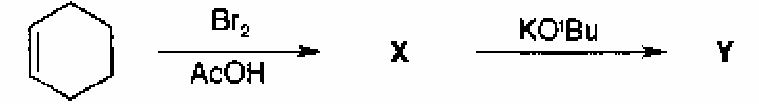
\includegraphics[width=0.6\textwidth]{fig5.png} 
\]
\begin{multicols}{2}
\begin{enumerate}
\item 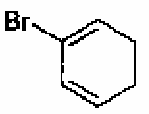
\includegraphics[width=0.2\textwidth]{fig6.png}
\item 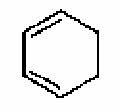
\includegraphics[width=0.2\textwidth]{fig7.png}
\item 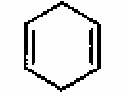
\includegraphics[width=0.2\textwidth]{fig8.png}
\item 
\includegraphics[width=0.2\textwidth]{fig9.png}
\end{enumerate}
\end{multicols}

% Q10
\item The ionization energy follows the order
\hfill{\brak{\text{GATE XL 2010}}}
\begin{multicols}{2}
\begin{enumerate}
\item O$_2^+$ $>$ O $>$ O$_2^-$ $>$ O$_2^{2-}$
\item O$_2^-$ $>$ O$_2^+$ $>$ O$_2$ $>$ O$_2^{2-}$
\item O$^-$ $>$ O$_2^-$ $>$ O$_2^+$ $>$ O$_2$
\item O$_2^{2-}$ $>$ O$_2^-$ $>$ O$_2$ $>$ O$_2^+$
\end{enumerate}
\end{multicols}

% Q11
\item Reaction of Na$_2$S with 2 equivalents of HCl produces a gas X. Solution of X in water is acidic in nature. X is
\hfill{\brak{\text{GATE XL 2010}}}
\begin{multicols}{2}
\begin{enumerate}
\item O$_2$
\item Cl$_2$
\item SO$_2$
\item H$_2$S
\end{enumerate}
\end{multicols}
k
% Q12
\item For a dilute solution of pho
sphorous acid in a pH 5 buffer, the predominant species is
\hfill{\brak{\text{GATE XL 2010}}}
\begin{multicols}{2}
\begin{enumerate}
\item  H$_3$PO$_3$
\item  H$_2$PO$_3^-$ 
\item   HPO$_3^{2-}$
\item PO$_3^{3-}$
\end{enumerate}
\end{multicols}

% Q13
\item The structure of phosphorous acid is
\hfill{\brak{\text{GATE XL 2010}}}
\begin{multicols}{2}
\begin{enumerate}
\item 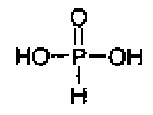
\includegraphics[width=0.25\textwidth]{fig10.png}
\item 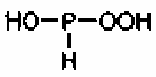
\includegraphics[width=0.25\textwidth]{fig11.png}
\item 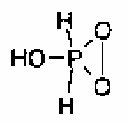
\includegraphics[width=0.25\textwidth]{fig12.png}
\item 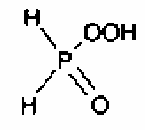
\includegraphics[width=0.25\textwidth]{fig13.png}
\end{enumerate}
\end{multicols}

\item The structure of X in the above reaction sequence is
\hfill{\brak{\text{GATE XL 2010}}}
\[
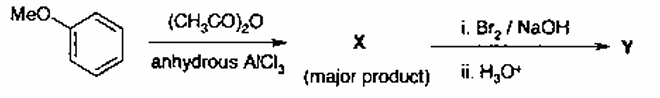
\includegraphics[width=0.6\textwidth]{fig14.png} 
\]

\begin{multicols}{2}
\begin{enumerate}
\item 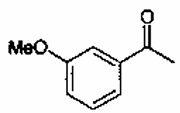
\includegraphics[width=0.25\textwidth]{fig15.png}
\item 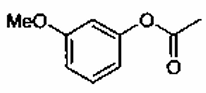
\includegraphics[width=0.25\textwidth]{fig16.png}
\item 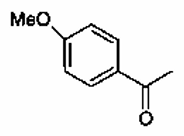
\includegraphics[width=0.25\textwidth]{fig17.png}
\item 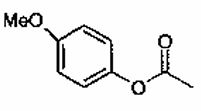
\includegraphics[width=0.25\textwidth]{fig18.png}
\end{enumerate}
\end{multicols}

% Q15
\item The structure of Y in the above reaction sequence is
\hfill{\brak{\text{GATE XL 2010}}}
\newpage
\begin{enumerate}
\begin{multicols}{2}
\item 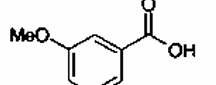
\includegraphics[width=0.25\textwidth]{fig19.png}
\item 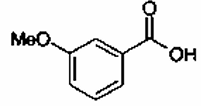
\includegraphics[width=0.25\textwidth]{fig20.png}
\item 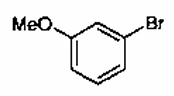
\includegraphics[width=0.25\textwidth]{fig21.png}
\item 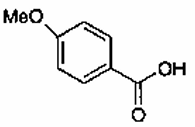
\includegraphics[width=0.25\textwidth]{fig22.png}
\end{multicols}
\end{enumerate}

\item Nucleolus is involved in the synthesis of 
\hfill{\brak{\text{GATE XL 2010}}}

\begin{enumerate}
\begin{multicols}{4}
\item rRNA
\item tRNA
\item DNA
\item mRNA
\end{multicols}
\end{enumerate}

\item In tryptophan operon, tryptophan acts as 
\hfill{\brak{\text{GATE XL 2010}}}

\begin{enumerate}
\begin{multicols}{4}
\item Repressor
\item Activator
\item Co-repressor
\item Co-activator
\end{multicols}
\end{enumerate}

\item Positive selection of T cells ensures 
\hfill{\brak{\text{GATE XL 2010}}}

\begin{enumerate}
\begin{multicols}{2}
\item MHC restriction
\item Self tolerance
\item TCR engagements
\item Activation by co-stimulatory signal
\end{multicols}
\end{enumerate}

\item A DNA-binding motif is 
\hfill{\brak{\text{GATE XL 2010}}}

\begin{enumerate}
\begin{multicols}{2}
\item Helix-loop-helix
\item Helix-turn-helix
\item Helical wheel
\item Loop-helix-loop
\end{multicols}
\end{enumerate}

\item Amino acids responsible for N-linked and O-linked glycosylation of proteins are 
\hfill{\brak{\text{GATE XL 2010}}}

\begin{enumerate}
\begin{multicols}{2}
\item Asparagine and Aspartic acid
\item Glutamine and Serine
\item Glutamic acid and Serine
\item Asparagine and Threonine
\end{multicols}
\end{enumerate}

\item One of the following compounds is NOT a neurotransmitter 
\hfill{\brak{\text{GATE XL 2010}}}

\begin{enumerate}
\begin{multicols}{2}
\item Dopamine
\item Glutamic acid
\item Histidine
\item Glycine
\end{multicols}
\end{enumerate}

\item Approximate molecular weight \brak{\text{kDa}} of the product after translation of a $390$ bases mRNA will be 
\hfill{\brak{\text{GATE XL 2010}}}

\begin{enumerate}
\begin{multicols}{4}
\item 48
\item 26
\item 39
\item 14
\end{multicols}
\end{enumerate}

\item Lineweaver-Burk plot is a plot of 
\hfill{\brak{\text{GATE XL 2010}}}

\begin{enumerate}
\begin{multicols}{2}
\item $\frac{1}{V_0}$ vs $\frac{1}{S}$
\item $V_0$ vs $\frac{1}{S}$
\item $V_0$ vs $S$
\item $\frac{1}{V_0}$ vs $S$
\end{multicols}
\end{enumerate}

\item A mixture of proteins \brak{\text{W, X, Y, Z}} elute from Sephadex G-200 column in the order W, X, Y, Z. The protein with maximum electrophoretic mobility on SDS-PAGE will be 
\hfill{\brak{\text{GATE XL 2010}}}

\begin{enumerate}
\begin{multicols}{4}
\item W
\item X
\item Y
\item Z
\end{multicols}
\end{enumerate}

\item Specific precursor for all prostaglandins is 
\hfill{\brak{\text{GATE XL 2010}}}

\begin{enumerate}
\begin{multicols}{2}
\item Oleic acid
\item Arachidonic acid
\item Palmitic acid
\item $\alpha$-Linolenic acid
\end{multicols}
\end{enumerate}

\item Chymotrypsin and lysozyme are involved respectively in 
\hfill{\brak{\text{GATE XL 2010}}}

\begin{enumerate}
\item[P] Removal of successive carboxyl terminal residues
\item[Q] Hydrolytic cleavage of peptide bond 
\item[R] Cleavage of glycosidic C-O bond
\item[S] Oxygen transport in bloo
\end{enumerate}

\begin{enumerate}
\begin{multicols}{2}
\item P, Q
\item Q, R
\item Q, S
\item R, S
\end{multicols}
\end{enumerate}

\item Match the items in Group 1 with those in Group 2 
\hfill{\brak{\text{GATE XL 2010}}}

\begin{table}[h]
\centering
\begin{tabular}{ll}
\textbf{Group 1} & \textbf{Group 2} \\
P. Isotype switching & 1. $V_H$ domain \\
Q. Clonal anergy & 2. Non-responsive to self antigen \\
R. Class II MHC & 3. Non-responsive TH cells \\
S. Self tolerance & 4. $\beta_2$ microglobulin \\
\end{tabular}
\caption*{}
\label{tab:q12}
\end{table}

\begin{enumerate}
\begin{multicols}{2}
\item P-1, Q-4, R-3, S-2
\item P-2, Q-4, R-1, S-3
\item P-1, Q-3, R-4, S-2
\item P-2, Q-1, R-3, S-4
\end{multicols}
\end{enumerate}

\item Multiple RNA polymerase transcribes a DNA template, unwinding about $1.5$ turns of DNA template per transcription bubble. From the structural information of classical B-DNA, how many transcription bubbles are possible for a $180$ base pair DNA molecule?
\hfill{\brak{\text{GATE XL 2010}}}

\begin{enumerate}
\begin{multicols}{4}
\item 12
\item 27
\item 6
\item 270
\end{multicols}
\end{enumerate}

\item Match the items in Group 1 with the most appropriate separation techniques in Group 2
\hfill{\brak{\text{GATE XL 2010}}}

\begin{table}[h]
\centering
\begin{tabular}{ll}
\textbf{Group 1} & \textbf{Group 2} \\
P. Mixture of glycine and albumin & 1. Gas chromatography \\
Q. Mixture of 20 and 60 kDa proteins & 2. Dialysis \\
R. Ribosomes from nuclear extract & 3. Affinity chromatography \\
S. Lectins & 4. Size exclusion chromatography \\
 & 5. Thin layer chromatography \\
 & 6. Cation exchange chromatography \\
\end{tabular}
\caption*{}
\label{tab:q14}
\end{table}

\begin{enumerate}
\begin{multicols}{2}
\item P-1, Q-4, R-3, S-5
\item P-5, Q-3, R-6, S-1
\item P-2, Q-4, R-3, S-5
\item P-6, Q-5, R-2, S-4
\end{multicols}
\end{enumerate}

\item In the two half reactions \\
Acetaldehyde + $2H^+ + 2e^- \to$ Ethanol \quad $\Delta E^\degree = -0.16\,V$ \\
NADH + $H^+ \to$ NAD$^+ + 2H^+ + 2e^-$ \quad $\Delta E^\degree = -0.32\,V$ \\
\brak{F = 23063 \text{ cal/V}} \\
The $\Delta G^\degree$ for coupled reaction will be 
\hfill{\brak{\text{GATE XL 2010}}}

\begin{enumerate}
\begin{multicols}{2}
\item +7,400 cal
\item -7,400 cal
\item -22,200 cal
\item +22,200 cal
\end{multicols}
\end{enumerate}

\item Match the parameters in Group 1 with the correct options in Group 2 
\hfill{\brak{\text{GATE XL 2010}}}

\begin{table}[h]
\centering
\begin{tabular}{ll}
\textbf{Group 1} & \textbf{Group 2} \\
P. $K_{cat}$ & 1. Catalytic efficiency of the enzyme \\
Q. $K_M$ & 2. Affinity of enzyme to the inhibitor \\
R. $K_I$ & 3. Affinity of enzyme to the substrate \\
S. $K_{cat}/K_M$ & 4. Maximum buffering rate \\
\end{tabular}
\caption*{}
\label{tab:q16}
\end{table}

\begin{enumerate}
\begin{multicols}{2}
\item P-3, Q-1, R-2, S-4
\item P-1, Q-2, R-3, S-4
\item P-3, Q-1, R-4, S-2
\item P-1, Q-4, R-2, S-3
\end{multicols}
\end{enumerate}

\item The rise per residue of $\alpha$-helix is about $1.5\,\mathring{A}$. A protein spans a $4nm$ bilayer $7$ times through its transmembrane $\alpha$-helical domain. Approximately, how many amino acid residues constitute the transmembrane domain of the protein 
\hfill{\brak{\text{GATE XL 2010}}}

\begin{enumerate}
\begin{multicols}{4}
\item 105
\item 451
\item 30
\item 190
\end{multicols}
\end{enumerate}

\item Match the proteins in Group 1 with their correct functions in Group 2 
\hfill{\brak{\text{GATE XL 2010}}}

\begin{table}[h]
\centering
\begin{tabular}{ll}
\textbf{Group 1} & \textbf{Group 2} \\
P. Shaker protein & 1. Inner membrane receptor \\
Q. Bacteriorhodopsin & 2. Active transport \\
R. Porin & 3. Voltage gated $K^+$ channel \\
S. ABC transporter & 4. Light driven $H^+$ pump \\
 & 5. Membrane fusion \\
 & 6. $\beta$-barrel simple diffusion channel \\
\end{tabular}
\caption*{}
\label{tab:q18}
\end{table}

\begin{enumerate}
\begin{multicols}{2}
\item P-4, Q-2, R-3, S-5
\item P-5, Q-3, R-4, S-6
\item P-6, Q-1, R-5, S-4
\item P-3, Q-4, R-6, S-2
\end{multicols}
\end{enumerate}

\item The metabolic disorders, Alkaptonuria and Phenylketonuria are caused by defects in the enzymes 
\hfill{\brak{\text{GATE XL 2010}}}
\begin{enumerate}
    \item[P] Glucose 6-phosphatase
    \item[Q] Phenylalanine hydroxylase
    \item[R] Homogentisate 1,2-dioxygenase
    \item[S] Tyrosinase
\end{enumerate}

\begin{enumerate}
\begin{multicols}{2}
\item Q, R
\item P, R
\item P, Q
\item Q, S
\end{multicols}
\end{enumerate}

\item Match the metabolic pathways in Group 1 with the corresponding enzymes in Group 2 
\hfill{\brak{\text{GATE XL 2010}}}

\begin{table}[h]
\centering
\begin{tabular}{ll}
\textbf{Group 1} & \textbf{Group 2} \\
P. $\beta$-oxidation & 1. Ribulose bisphosphate carboxylase \\
Q. Glycolysis & 2. Phosphofructokinase 1 \\
R. Gluconeogenesis & 3. Phosphoenol pyruvate carboxykinase \\
S. Calvin cycle & 4. Thiolase \\
 & 5. Phosphofructokinase 2 \\
\end{tabular}
\caption*{}
\label{tab:q20}
\end{table}

\begin{enumerate}
\begin{multicols}{2}
\item P-4, Q-2, R-3, S-5
\item P-3, Q-2, R-4, S-1
\item P-3, Q-1, R-5, S-2
\item P-4, Q-2, R-3, S-1
\end{multicols}
\end{enumerate}

\item When changes in the phenotype or gene expression occur without changes in the underlying DNA sequence, the phenomenon is called 
\hfill{\brak{\text{GATE XL 2010}}}

\begin{enumerate}
\begin{multicols}{2}
\item Mutation
\item Eugenics
\item Epigenetics
\item Epistasis
\end{multicols}
\end{enumerate}

\item A population growing exponentially can be described by the differential equation $dN/dt = rN$, where $dN/dt$ represents the rate at which the whole population grows, $N$ is the size of the population, $r$ is the intrinsic rate of increase, and $t$ is time. According to this equation, the per capita rate of growth is 
\hfill{\brak{\text{GATE XL 2010}}}

\begin{enumerate}
\begin{multicols}{2}
\item Highest at large $N$
\item Constant
\item Lowest at large $N$
\item Highest at small $N$
\end{multicols}
\end{enumerate}

\item Which one of the following is NOT a plant hormone? 
\hfill{\brak{\text{GATE XL 2010}}}

\begin{enumerate}
\begin{multicols}{2}
\item Abscisic acid
\item Brassinosteroid
\item Ethylene
\item Cytokine
\end{multicols}
\end{enumerate}

\item \textit{Arabidopsis} and rice have diploid chromosome numbers of 10 and 24, respectively. Assuming no crossing over taking place, genetic variation among $F_2$ individuals in a genetic cross is likely to be 
\hfill{\brak{\text{GATE XL 2010}}}

\begin{enumerate}
\begin{multicols}{2}
\item Same in both species but not zero
\item More in \textit{Arabidopsis}
\item More in rice
\item Zero in both species
\end{multicols}
\end{enumerate}

\item Which of the following statements is CORRECT? 
\hfill{\brak{\text{GATE XL 2010}}}

\begin{enumerate}
\item Plants adapted to cold environment have higher ratio of ``unsaturated to saturated'' fatty acids in their membrane compared to those adapted to hot environment
\item Plants adapted to cold environment have lower ratio of ``unsaturated to saturated'' fatty acids in their membrane compared to those adapted to hot environment
\item Plants adapted to cold and hot environment have same ratio of ``unsaturated to saturated'' fatty acids in their membrane compared to those adapted to hot environment
\item There are only saturated fatty acids in the membrane
\end{enumerate}

\item A sign is hammered into a tree trunk 2 meters above the tree’s base. If the tree is 10 meters tall and elongates 1 meter each year, how high will the sign be after 10 years? 
\hfill{\brak{\text{GATE XL 2010}}}

\begin{enumerate}
\begin{multicols}{2}
\item 12 meters
\item 10 meters
\item 4 meters
\item 2 meters
\end{multicols}
\end{enumerate}

\item In the arrangement of floral parts in a bud, identify the INCORRECT statement 
\hfill{\brak{\text{GATE XL 2010}}}

\begin{enumerate}
\item Valvate: where the petals or sepals do not overlap but simply touch one another by their margins
\item Scarious: petals rough and harsh to touch
\item Epicalyx: an extra whorl calyx found in some flowers outside the calyx
\item Imbricate: where sepals and petals overlap each other at the margin
\end{enumerate}

\item The possible genotypes of endosperms borne on a heterozygous (Rr) plant will be
\hfill{\brak{\text{GATE XL 2010}}}

\begin{enumerate}
\begin{multicols}{2}
\item RRR, Rrr, Rrr, rr
\item RRr, Rrr
\item RR, Rr, rr
\item Rr
\end{multicols}
\end{enumerate}

\item The amount of chemical energy available to consumers in an ecosystem is best represented by
\hfill{\brak{\text{GATE XL 2010}}}

\begin{enumerate}
\begin{multicols}{2}
\item Gross primary production
\item Net primary production
\item Respiration
\item Photosynthesis
\end{multicols}
\end{enumerate}

\item Free radical scavenging activity of a medicinally important plant extract can be quantified by 
\hfill{\brak{\text{GATE XL 2010}}}

\begin{enumerate}
\item ABTS (2,${2'}$-azino-bis-(3-ethyl benzothiazoline-6-sulphonic acid)) method
\item Bradford method
\item Walkley and Black method
\item Kjeldahl method
\end{enumerate}

\item \textbf{Identify the CORRECT statements from the following} 
\hfill{\brak{\text{GATE XL 2010}}}

P. Lenticels are the small pores present on the surface of the stem or branches of woody plants. \\
Q. Glyoxysomes contain chlorophyll molecules in their thylakoid membranes. \\
R. The enzyme ribulose 1,5 bisphosphate carboxylase is otherwise known as carboxydismutase. \\
S. 18 ATP and 12 NADPH molecules are utilized for fixing 6 molecules of CO$_2$ in the dark reaction of photosynthesis.

\begin{enumerate}
\begin{multicols}{2}
\item P, Q
\item P, R
\item Q, R
\item P, S
\end{multicols}
\end{enumerate}

\item \textbf{Match the following} 
\hfill{\brak{\text{GATE XL 2010}}}

\begin{center}
\begin{tabular}{lll}
\textbf{Group I} & \textbf{Group II} & \textbf{Group III} \\
P. Sorghum & 1. Gossypol & i. Protein \\
Q. Castor & 2. Strychnine & ii. Glycosidic conjugate \\
R. Mushroom & 3. Durin & iii. Alkaloid \\
S. Cotton & 4. Bungarotoxin & iv. Polyphenol \\
& 5. Ricin & v. Lipid \\
& 6. $\alpha$-Amanitin & vi. Cyclic peptide
\end{tabular}
\end{center}

\begin{enumerate}
\begin{multicols}{2}
\item P-3,i; Q-5,i; R-6,vi; S-1,iv
\item P-2,ii; Q-4,iv; R-1,iii; S-6,v
\item P-2,vi; Q-5,v; R-1,iv; S-6,i
\item P-2,ii; Q-3,iii; R-4,iv; S-1,v
\end{multicols}
\end{enumerate}

\item Name the structures given below in the order of their appearance and identify corresponding glycosidic linkages

\begin{figure}[H]

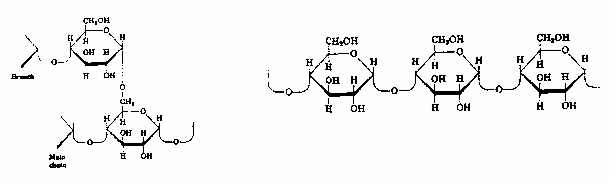
\includegraphics[width=0.9\columnwidth]{fig24.png}
\caption*{}
\label{fig:q16}
\end{figure}
\hfill{\brak{\text{GATE XL 2010}}}
\begin{enumerate}
\begin{multicols}{2}
\item Amylose, Cellulose; $\alpha\brak{1 \to 4}$, $\beta\brak{1 \to 6}$
\item Cellulose, Dextran; $\beta\brak{2 \to 4}$, $\alpha\brak{3 \to 6}$
\item Starch, Cellulose; $\alpha\brak{1 \to 6}$, $\alpha\brak{1 \to 4}$
\item Amylopectin, Amylose; $\alpha\brak{1 \to 6}$, $\alpha\brak{1 \to 4}$
\end{multicols}
\end{enumerate}

\item Identify the \textbf{CORRECT} statements

\text{In \textit{Arabidopsis}, vernalization is associated with}

P. Chromatin modification at the \textit{FLC \brak{FLOWERING LOCUS C}} locus \\
Q. Degradation of the FLC protein \\
R. Inactivating the FLC protein by post-translational modification \\
S. Down-regulation of \textit{FLC} transcript
\hfill{\brak{\text{GATE XL 2010}}}
\begin{enumerate}
\begin{multicols}{2}
\item Q, S
\item P, S
\item P, R
\item Q, R
\end{multicols}
\end{enumerate}


\item Which of the following statements in plant respiration are \textbf{CORRECT}?
\begin{enumerate}
    

\item[P] The oxidative Pentose Phosphate Pathway can accomplish the oxidation of glucose in the stroma of mitochondria \\
\item[Q] ATP is produced in the reaction step of TCA cycle catalyzed by succinyl CoA synthetase \\
\item[R] In addition to Cytochrome c oxidase, an alternative oxidase enzyme resistant to cyanide reduces oxygen molecule in the electron transport system \\
\item[S] In Glyoxylate cycle acetyl CoA reacts with citrate to form $\alpha$-keto glutarate
\end{enumerate}
\hfill{\brak{\text{GATE XL 2010}}}
\begin{enumerate}
\begin{multicols}{2}
\item P, R
\item P, Q
\item Q, R
\item Q, S
\end{multicols}
\end{enumerate}

\item Study the following diagram depicting the plant cell cycle and match the following
\hfill{\brak{\text{GATE XL 2010}}}
\begin{figure}[H]
\centering
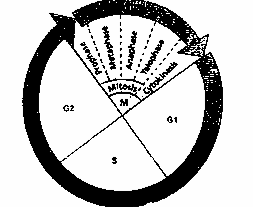
\includegraphics[width=0.4\columnwidth]{fig25.png}
\caption*{}
\label{fig:q19}
\end{figure}

\begin{table}[h!]
\centering
\begin{tabular}{|c|c|}
\hline
\textbf{Stages of cell cycle} & \textbf{Type of cyclin} \\
\hline
P. Late G1-phase & 1. Cyclin B \\
Q. Beginning of S-phase & 2. Cyclin E \\
R. Prior to mitotic phase & 3. S-Cyclin \\
S. Early G1-phase & 4. Cyclin D \\
\hline
\end{tabular}
\caption*{}
\label{tab:q19}
\end{table}

\begin{enumerate}
\begin{multicols}{2}
\item P-4, Q-3, R-1, S-2
\item P-2, Q-3, R-1, S-4
\item P-1, Q-4, R-3, S-2
\item P-3, Q-1, R-2, S-4
\end{multicols}
\end{enumerate}



\item In the context of plant development, which of the following statements are \textbf{CORRECT}?
\begin{enumerate}
     
\item[P] Cell migration is absent \\
\item[Q] Apoptosis plays a major role \\
\item[R] Pattern formation continues throughout life \\
\item[S] Homeotic changes are caused by mutations in non-homeodomain proteins
\end{enumerate}
\hfill{\brak{\text{GATE XL 2010}}}
\begin{enumerate}
\begin{multicols}{2}
\item P, Q, R
\item Q, R, S
\item P, Q, S
\item P, R, S
\end{multicols}
\end{enumerate}

 \item Identify the correct match

    \begin{minipage}{0.6\textwidth}
        \textbf{Group I \brak{\text{Anther}}}
        \begin{figure}[H]
            \centering
            \begin{tabular}{cc}
                 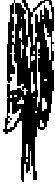
\includegraphics[width=0.15\columnwidth]{fig26.png} & 
\includegraphics[width=0.2\columnwidth]{fig27.png} \\
                 P & Q \\[1em]
                 
\includegraphics[width=0.2\columnwidth]{fig28.png} & 
\includegraphics[width=0.2\columnwidth]{fig29.png} \\
                 R & S
            \end{tabular}
            \caption*{}
            \label{fig:q13group}
        \end{figure}
    \end{minipage}%
    \begin{minipage}{0.4\textwidth}
        \textbf{Group II \brak{\text{Type of fixation}}}
        \begin{enumerate}
            \item Basifixed
            \item Longitudinal
            \item Dorsifixed
            \item Adenate
            \item Porous
            \item Versatile
        \end{enumerate}
    \end{minipage}

    \hfill{\brak{\text{GATE XL 2010}}}

    \begin{enumerate}
        \begin{multicols}{4}
            \item P-$1$, Q-$4$, R-$6$, S-$3$
            \item P-$2$, Q-$3$, R-$5$, S-$6$
            \item P-$1$, Q-$2$, R-$6$, S-$5$
            \item P-$4$, Q-$3$, R-$5$, S-$6$
        \end{multicols}
    \end{enumerate}

    \item From the structures given below, identify the compounds

    \begin{minipage}{0.6\textwidth}
        \textbf{Group I \brak{\text{Structure}}}
        \begin{figure}[H]
            \centering
            \begin{tabular}{cc}
                 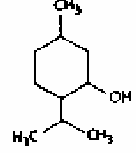
\includegraphics[width=0.3\columnwidth]{fig30.png} & 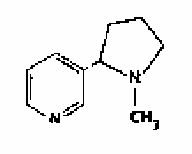
\includegraphics[width=0.3\columnwidth]{fig31.png} \\
                 P & Q \\[1em]
                 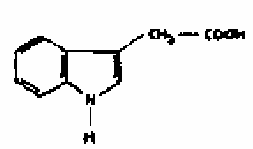
\includegraphics[width=0.3\columnwidth]{fig32.png} & 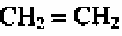
\includegraphics[width=0.3\columnwidth]{fig33.png} \\
                 R & S
            \end{tabular}
            \caption*{}
            \label{fig:q14group}
        \end{figure}
    \end{minipage}%
    \begin{minipage}{0.4\textwidth}
        \textbf{Group II \brak{\text{Compound}}}
        \begin{enumerate}
            \item Ethylene
            \item Indole butyric acid
            \item Nicotine
            \item Indole acetic acid
            \item Gibberellic acid
            \item Menthol
        \end{enumerate}
    \end{minipage}

    \hfill{\brak{\text{GATE XL 2010}}}

    \begin{enumerate}
        \begin{multicols}{4}
            \item P-$6$, Q-$3$, R-$4$, S-$1$
            \item P-$5$, Q-$2$, R-$3$, S-$1$
            \item P-$4$, Q-$3$, R-$2$, S-$6$
            \item P-$1$, Q-$2$, R-$5$, S-$6$
        \end{multicols}
    \end{enumerate}

\item Regarding the relationships between two organisms in an ecosystem, match the following

\begin{table}[h!]
\centering
\begin{tabular}{|c|c|}
\hline
\textbf{Group I (Relationship)} & \textbf{Group II (Definition)} \\
\hline
P. Commensalism & 1. Both organisms are benefited \\
Q. Mutualism & 2. One impeding the success of the other \\
R. Parasitism & 3. One organism benefits but the other is unaffected \\
S. Amensalism & 4. One benefited, other is harmed \\
\hline
\end{tabular}
\caption*{}
\label{tab:q15}
\end{table}
\hfill{\brak{\text{GATE XL 2010}}}
\begin{enumerate}
\begin{multicols}{2}
\item P-3, Q-2, R-4, S-1
\item P-2, Q-3, R-4, S-1
\item P-3, Q-1, R-4, S-2
\item P-1, Q-4, R-3, S-2
\end{multicols}
\end{enumerate}

\item An electron microscope has higher resolution as compared to the light microscope. This is because

\hfill{\brak{\text{GATE XL 2010}}}

\begin{enumerate}
\item the wavelength of an electron is longer than the wavelength of light
\item the wavelength of an electron is shorter than the wavelength of light
\item the electrons can penetrate the sample better
\item they use different stains
\end{enumerate}

\item Bacterial cell lysis by lysozyme is due to the

\hfill{\brak{\text{GATE XL 2010}}}

\begin{enumerate}
\item hydrolysis of $\alpha\brak{1 \to 4}$-glycosidic bonds between the N-acetylglucosamine and N-acetylmuramic acid
\item inhibition of cell wall synthesis
\item hydrolysis of pentapeptide bridges
\item hydrolysis of $\beta\brak{1 \to 4}$-glycosidic bonds between the N-acetylglucosamine and N-acetylmuramic acid
\end{enumerate}

\item The recombination frequencies between three genes x, y and z are as follows$\colon$

x-y$\colon$ $2.6\%$, y-z$\colon$$1.4\%$ and x-z$\colon$ $1.2\%$. Then the gene order is

\hfill{\brak{\text{GATE XL 2010}}}

\begin{enumerate}
\begin{multicols}{2}
\item x-y-z
\item x-z-y
\item y-x-z
\item z-x-y
\end{multicols}
\end{enumerate}

\item A mutant phenotype due to a nonsense mutation can be rescued by a mutation in tRNA gene. This rescue is an example of

\hfill{\brak{\text{GATE XL 2010}}}

\begin{enumerate}
\begin{multicols}{2}
\item induced mutation
\item suppressor mutation
\item spontaneous mutation
\item deletion mutation
\end{multicols}
\end{enumerate}

\item Ames test is performed to detect

\hfill{\brak{\text{GATE XL 2010}}}

\begin{enumerate}
\begin{multicols}{2}
\item mutagen
\item pH
\item nutrient stress
\item salinity
\end{multicols}
\end{enumerate}

\item Wild type E. coli forms purple colored colonies on EMB-lactose plate. This is due to

\hfill{\brak{\text{GATE XL 2010}}}

\begin{enumerate}
\begin{multicols}{2}
\item increase in pH of the medium
\item decrease in pH of the medium
\item secretion of purple colored pigment
\item secretion of $\beta$-galactosidase
\end{multicols}
\end{enumerate}

\item The resistance of a lambda lysogenic E. coli to re-infection by lambda is mediated by

\hfill{\brak{\text{GATE XL 2010}}}

\begin{enumerate}
\begin{multicols}{2}
\item blocking entry of the incoming lambda DNA
\item degrading the incoming lambda DNA
\item blocking transcription of the incoming lambda DNA
\item triggering mutation of the lambda receptor of the host
\end{multicols}
\end{enumerate}

\item Pasteurization of milk is carried out by

\hfill{\brak{\text{GATE XL 2010}}}

\begin{enumerate}
\begin{multicols}{2}
\item boiling for 5 min
\item heating at $72\degree$C for 30 min
\item heating at $63\degree$C for 15 min
\item heating at $63\degree$C for 30 min
\end{multicols}
\end{enumerate}

\item A growing bacterial culture with a doubling time of 20 min reaches cell density of $2 \times 10^8$ cells/ml in 3 hours. How much time would it take to reach the cell density of $1 \times 10^9$ cells/ml?

\hfill{\brak{\text{GATE XL 2010}}}

\begin{enumerate}
\begin{multicols}{2}
\item 200 min
\item 180 min
\item 160 min
\item 90 min
\end{multicols}
\end{enumerate}

\item The quickest way to determine bacterial growth in terms of viable cells is through

\hfill{\brak{\text{GATE XL 2010}}}

\begin{enumerate}
\begin{multicols}{2}
\item Most probable number (MPN) technique
\item Spread plate method
\item Pour plate method
\item Slide culture technique
\end{multicols}
\end{enumerate}

\item Match the scientist from Group I with the corresponding contribution listed in Group II

\hfill{\brak{\text{GATE XL 2010}}}

Group I:
P. Robert Koch \\
Q. Walter Hesse \\
R. Louis Pasteur \\
S. Ferdinand Cohn

Group II:
1. Discovery of endospores \\
2. Disproved spontaneous generation \\
3. Discovery of causative agent of tuberculosis \\
4. Use of agar as solid media \\
5. Invention of microscope

\begin{enumerate}
\begin{multicols}{2}
\item P-5, Q-1, R-3, S-2
\item P-3, Q-4, R-1, S-5
\item P-3, Q-4, R-2, S-5
\item P-3, Q-4, R-2, S-1
\end{multicols}
\end{enumerate}

\item Superantigens elicit a very strong T cell response because they

\hfill{\brak{\text{GATE XL 2010}}}

\begin{enumerate}
\begin{multicols}{2}
\item bind to the specific antigen binding site on the T cell receptors (TCR)
\item bind to the site on T cell receptor (TCR) that is outside the antigen-specific binding site
\item directly activate the T cell without the help of antigen presenting cells
\item directly induce cytokine secretion by macrophages
\end{multicols}
\end{enumerate}

\item MHC-I groove can be loaded with peptides of only 8–10 amino acids because

\hfill{\brak{\text{GATE XL 2010}}}

\begin{enumerate}
\begin{multicols}{2}
\item MHC-I groove is closed on both ends
\item fragments of only 8–10 amino acids are generated in MHC-I bearing cells
\item $\beta_2$-microglobulin of MHC-I prevents binding of large peptides to MHC-I
\item pI of polypeptides of MHC-I prevents binding of 8–10 amino acid long peptides to MHC-I
\end{multicols}
\end{enumerate}

\item In a $lacO^c$ $lacIz^{+}$ / lacO$^{+}$ lacI$z^{-}$ partial diploid, of the two lacZ enzymes, only the mutant enzyme \brak{lacZ^{-}} is synthesized constitutively. This observation shows that lacO$^c$ mutation is

\hfill{\brak{\text{GATE XL 2010}}}

\begin{enumerate}
\begin{multicols}{2}
\item trans-dominant
\item trans-recessive
\item cis-dominant
\item cis-recessive
\end{multicols}
\end{enumerate}

\item Which one of the following events occurs in prokaryotes but NOT in eukaryotes?

\hfill{\brak{\text{GATE XL 2010}}}

\begin{enumerate}
\begin{multicols}{2}
\item Phosphorylation
\item RNA polymerase and promoter interaction
\item Control of transcription by attenuation
\item Formation of Okazaki fragments
\end{multicols}
\end{enumerate}

 \item Match the pathogen in Group I with the corresponding disease in Group II
    
    \begin{minipage}[t]{0.5\textwidth}
        \textbf{Group I} \\
        P. Bacteria \\
        Q. Virus \\
        R. Fungi \\
        S. Protozoa
    \end{minipage}%
    \begin{minipage}[t]{0.5\textwidth}
        \textbf{Group II} \\
        1. Measles \\
        2. Candidiasis \\
        3. Malaria \\
        4. Tetanus \\
        5. Acute apicomplexan encephalitis \\
        6. Tuberculosis
    \end{minipage}

    \hfill{\brak{\text{GATE XL 2010}}}

    \begin{enumerate}
        \begin{multicols}{2}
            \item \brak{\text{P-1, Q-2, R-4, S-5}}
            \item \brak{\text{P-4, Q-6, R-2, S-3}}
            \item \brak{\text{P-5, Q-1, R-6, S-2}}
            \item \brak{\text{P-6, Q-1, R-2, S-3}}
        \end{multicols}
    \end{enumerate}

    \item A bacterial culture was diluted $1000$ fold and $0.1$ ml of this diluted sample was spread per plate on nutrient agar. In a triplicate run, the number of colonies formed is $121$, $93$ and $86$. The number of colony forming units/ml in the original bacterial culture is

    \hfill{\brak{\text{GATE XL 2010}}}

    \begin{enumerate}
        \begin{multicols}{4}
            \item ${10^5}$
            \item ${10^6}$
            \item ${10^7}$
            \item ${10^8}$
        \end{multicols}
    \end{enumerate}

    \item Match the microorganism in Group I with the application in Group II
    
    \begin{minipage}[t]{0.5\textwidth}
        \textbf{Group I} \\
        P. Aspergillus oryzae \\
        Q. Brevibacterium flavum \\
        R. Candida lipolytica \\
        S. Saccharomyces cerevisiae \\
        T. Rhizobium meliloti
    \end{minipage}%
    \begin{minipage}[t]{0.5\textwidth}
        \textbf{Group II} \\
        1. Metal ore leaching \\
        2. Glucoamylase producer \\
        3. Biopesticide \\
        4. Glutamic acid producer \\
        5. Penicillin producer \\
        6. Symbiotic nitrogen fixer
    \end{minipage}

    \hfill{\brak{\text{GATE XL 2010}}}

    \begin{enumerate}
        \begin{multicols}{2}
            \item \brak{\text{P-1,Q-4,R-6,S-5,T-2}}
            \item \brak{\text{P-1,Q-4,R-5,S-3,T-6}}
            \item \brak{\text{P-2,Q-4,R-1,S-3,T-6}}
            \item \brak{\text{P-6,Q-2,R-3,S-5,T-1}}
        \end{multicols}
    \end{enumerate}

    \item A microbe is grown normally on glucose or on glycerol but not on acetate. The most likely metabolic pathway that is defective in the microbe is

    \hfill{\brak{\text{GATE XL 2010}}}

    \begin{enumerate}
        \begin{multicols}{2}
            \item \brak{\text{Glyoxalate cycle}}
            \item \brak{\text{Hexose monophosphate shunt}}
            \item \brak{\text{Kreb's cycle}}
            \item \brak{\text{Entner-Doudoroff pathway}}
        \end{multicols}
    \end{enumerate}

    \item Match the resistance mechanism in Group I with the antibiotic in Group II
    
    \begin{minipage}[t]{0.5\textwidth}
        \textbf{Group I} \\
        P. $\beta$-Lactamases \\
        Q. Enhanced folate metabolism \\
        R. Drug efflux \\
        S. Overproduction of the drug \\
        T. Mutant RNA polymerase
    \end{minipage}%
    \begin{minipage}[t]{0.5\textwidth}
        \textbf{Group II} \\
        1. Aminoglycosides \\
        2. Penicillins \\
        3. Sulfa drugs \\
        4. Tetracyclines \\
        5. Nalidixic acid \\
        6. Rifamycin
    \end{minipage}

    \hfill{\brak{\text{GATE XL 2010}}}

    \begin{enumerate}
        \begin{multicols}{2}
            \item \brak{\text{P-1,Q-2,R-3,S-4,T-6}}
            \item \brak{\text{P-2,Q-3,R-4,S-5,T-6}}
            \item \brak{\text{P-2,Q-3,R-4,S-1,T-6}}
            \item \brak{\text{P-1,Q-2,R-3,S-4,T-6}}
        \end{multicols}
    \end{enumerate}

\item From the perspective of developmental origin, which of the following structures is homologous to a tortoise shell?

\hfill{\brak{\text{GATE XL 2010}}}

\begin{enumerate}
\begin{multicols}{1}
\item Exoskeleton of a lobster
\item Bones of a fish
\item Skull of humans
\item Feathers of birds
\end{multicols}
\end{enumerate}

\item Acoelomates are characterized by

\hfill{\brak{\text{GATE XL 2010}}}

\begin{enumerate}
\begin{multicols}{1}
\item the absence of cavity surrounding the internal organs
\item the presence of huge body cavity, as in case of terrestrial animals
\item the presence of air sacs, as in case of birds
\item the absence of brain in a group of extinct species
\end{multicols}
\end{enumerate}

\item Identify the phylum that is characterized by the animals that have segmented appendages.

\hfill{\brak{\text{GATE XL 2010}}}

\begin{enumerate}
\begin{multicols}{4}
\item Cnideria
\item Porifera
\item Arthropoda
\item Mollusca
\end{multicols}
\end{enumerate}

\item Which one of the following is the smallest biological unit capable of evolving over time?

\hfill{\brak{\text{GATE XL 2010}}}

\begin{enumerate}
\begin{multicols}{1}
\item A cell
\item An individual organism
\item A population
\item A species
\end{multicols}
\end{enumerate}

\item In case of parasites that require multiple hosts to complete their life cycle, what does definitive host mean?

\hfill{\brak{\text{GATE XL 2010}}}

\begin{enumerate}
\begin{multicols}{1}
\item It is the host that harbors the sexual stages of the parasite.
\item It is the host in which the parasite reproduces asexually.
\item It is the host in which the parasite feeds.
\item It is the host in which the parasite remains in a dormant stage.
\end{multicols}
\end{enumerate}

\item Enzymes catalyze biochemical reactions by

\hfill{\brak{\text{GATE XL 2010}}}

\begin{enumerate}
\begin{multicols}{1}
\item sequestering the product\brak{\text{s}}
\item decreasing the $\Delta G$ of the reaction
\item increasing the $\Delta G$ of the reaction
\item stabilizing the transition state of the reaction
\end{multicols}
\end{enumerate}

\item Which one of the following results from Mendel's monohybrid cross is the strongest evidence against the blending theory?

\hfill{\brak{\text{GATE XL 2010}}}

\begin{enumerate}
\begin{multicols}{1}
\item $3 \colon 1$ ratio of phenotypes in the F$1$ generation
\item All progeny of the F$1$ generation exhibited the dominant phenotype
\item The recessive phenotype showed up in the F$2$ progeny
\item The observation of incomplete dominance
\end{multicols}
\end{enumerate}

\item In the context of cell differentiation, lateral inhibition is referred to as the

\hfill{\brak{\text{GATE XL 2010}}}

\begin{enumerate}
\begin{multicols}{1}
\item formation of two distinct cell types within a uniform field
\item inhibition of formation of a distinct cell type next to an existing cell type
\item inhibition of stem cells towards self-renewal
\item inhibition of erythropoiesis in the lateral plate mesoderm
\end{multicols}
\end{enumerate}

\item As compared to peptide hormones, steroid hormones take more time to activate a cellular response because

\hfill{\brak{\text{GATE XL 2010}}}

\begin{enumerate}
\item steroid hormones show non-specific binding with diverse sets of receptors
\item steroid hormone acts through a receptor which is a transcription factor
\item cells that respond to steroid hormones are dormant in nature
\item peptide hormones are not transported through plasma while steroid hormones are
\end{enumerate}

\item In allopatric mode of speciation, a new species forms due to

\hfill{\brak{\text{GATE XL 2010}}}

\begin{enumerate}
\item Geographic isolation
\item Genetic drift
\item Formation of a few fertile individuals that can not mate with other members of the same species living in the same geographical area
\item The formation of allopolyploid condition
\end{enumerate}

\item Neurogen \brak{\text{Ngn}} a newly discovered protein in chicken, is produced by the notochord and the floor plate \brak{\text{FP}}. Ngn induces cells of the neural tube \brak{\text{NT}} to become neurons. It is known that from ventral to dorsal direction cells at different levels give rise to distinct types of neuronal cells. Which of the following observations will cast a doubt in the claim that Ngn is a morphogen?

\hfill{\brak{\text{GATE XL 2010}}}

\begin{enumerate}
\item Ngn is a cytosolic protein
\item Artificial mis-expression of Ngn at identical level through out NT does not affect the neuronal cell types formed in the NT
\item Ngn is an integral membrane protein
\item All of the above
\end{enumerate}

\item An alien species has been discovered with very similar genetic makeup as that of the existing species on planet earth with certain differences. The genetic material of this new species is referred to as DNA*. The building blocks of the genetic material is known as Nucleotide*. The proteins of the new species \brak{\text{Protein*}} is made up of Amino Acids*.\\

It has also been discovered that the new species has $5$ distinct Nucleotide* as opposed to the four for species on planet earth. The new species has $40$ different Amino Acids* as opposed to the $20$ for species of planet earth. What should be the codon length for this new species (the same for species of planet earth is $3$)? It may be assumed that the average codon degeneracy of the new species is very similar to that of species of planet earth.

\hfill{\brak{\text{GATE XL 2010}}}

\begin{enumerate}
\begin{multicols}{4}
\item $2$
\item $3$
\item $4$
\item $5$
\end{multicols}
\end{enumerate}

\item Which one of the following options is NOT a viable strategy for developing a female contraceptive\brak{} The administration of

\hfill{\brak{\text{GATE XL 2010}}}

\begin{enumerate}
\item a combination of synthetic progesterone and estrogen
\item synthetic progesterone alone
\item ormeloxifene - a selective estrogen receptor modulator
\item a synthetic oxytocin
\end{enumerate}

\item In the field of community ecology, the term \brak{\text{competitive exclusion}} refers to two species that cannot co-exist

\hfill{\brak{\text{GATE XL 2010}}}

\begin{enumerate}
\item in a community if the niches are identical
\item in two different communities if the niches are identical
\item if the ecosystem is imbalanced
\item in the event of a volcanic eruption
\end{enumerate}

  \item During immune response, more potent humoral immunity against the antigen appears earlier than the primary response. Which one of the following is the primary reason for this phenomenon?

    \hfill{\brak{\text{GATE XL 2010}}}
    \begin{enumerate}
        \item Affinity of antibody molecules produced by B cells is weaker than that of T cells.
        \item Memory cells have a longer life span than that of T cells.
        \item B-cell activation requires helper T cells.
        \item Thymus selection more rapidly enhances the T cell population than B cell population.
    \end{enumerate}

    \item Oceans have enormous impact on the biosphere. Identify which one of the following factors is NOT influenced by the marine biome.

    \hfill{\brak{\text{GATE XL 2010}}}
    \begin{enumerate}
        \item $CO_2$ level in the atmosphere.
        \item Global air temperature and wind patterns.
        \item pH of the fresh water bodies.
        \item Oxygen level in the biosphere.
    \end{enumerate}

    \item Certain lung fishes that live in small stagnant fresh water pools produce urea as a nitrogenous waste. What is the advantage of this adaptation?

    \hfill{\brak{\text{GATE XL 2010}}}
    \begin{enumerate}
        \item Urea forms precipitates and does not accumulate in the surrounding water.
        \item Lung fish do not find enough water for production of ammonia and hence the nitrogenous waste is converted to urea.
        \item The surrounding water makes the pool uninhabitable to the predators of the lung fish.
        \item Urea requires much less energy for its synthesis than ammonia.
    \end{enumerate}

    \item Hamilton's rule measures the probability of whether or not natural selection would favor an altruistic act. Which one of the following statements best explains Hamilton's rule. Natural selection would favor an altruistic act only when

    \hfill{\brak{\text{GATE XL 2010}}}
    \begin{enumerate}
        \item the receiver and not the altruist is benefited.
        \item the benefit to the receiver is higher than the cost of the altruist.
        \item the benefit to the receiver, reduced by the coefficient of relatedness, exceeds the cost to the altruist.
        \item the altruist survives in an altruistic act to save his/her related individuals.
    \end{enumerate}

    \item In a cross between plants with purple- and white-colored flowers, the following results were obtained in the $F_2$ generation from a single test cross. The numbers of different colored flowers were $900$ purple, $300$ lilac, $400$ white; $150$ yellow, $200$ blue, $245$ greenish yellow, $300$ green; and light blue; $400$ red, $200$ indigo, $253$ purple; and $198$ dark purple. These data support which one of the following conclusions.

    \hfill{\brak{\text{GATE XL 2010}}}
    \begin{enumerate}
        \item Flower color in this species does not follow Mendelian inheritance.
        \item It is a polygenic inheritance.
        \item Colors are co-dominant in this species.
        \item Flower color in this species is determined by multiple genes.
    \end{enumerate}

    \item Which one of the following is most crucial for the success of vaccination?

    \hfill{\brak{\text{GATE XL 2010}}}
    \begin{enumerate}
        \item Antigen presentation by T-helper cells.
        \item Complement system.
        \item Presence of long-lived antigen specific lymphocytes.
        \item Phagocytosis of the cells in the lymphoid tissue.
    \end{enumerate}


\end{enumerate}
\end{document} 
